\part{Results}
\chapter{Results}
\section{Imaging live cells}
For the study described in paper I we used cells of two species of cyanobacteria as a sample (Cyanobium gracile and Synechococcus elongatus). Cyanobacteria are photosynthetic bacteria that can be found in almost any habitat on earth, ranging from hot volcanic areas to cold polar ice caps. They play an important role in the global carbon cycle. In a 25 day cycle an algal bloom of 1000 $km^2$ can sequester around 22,000 tonnes of atmospheric carbon into organic carbon before cyanophages caused the bloom to collapse.
 
Cyanobium gracile cells were selected for their small size, their robustness with respect to the injection procedure, and convenient autofluorenscence properties to assess cell viability. Solitary C. gracile and S. elongatus cells have an oval-to-cylindrical shape, and vary in size between 0.25-0.4 $\mu$m in diameter and 0.4-4.0 $\mu$m in length [Komarek]. Cell divide symmetrically by binary fission. The two daughter cells separate from each other after reaching the size and shape of the mother cell [Komarek2]. We used non-synchronised cell cultures undergoing active growth providing cells in various stages of their cell cycle. 

The experiments described in paper I was carried out at the atomic, molecular, and optical science (AMO) endstation at LCLS at 512 eV (2.40 nm) and 1100 eV (1.13 nm) photon energy.  Figure \ref{fig:ExperimentalSetup} shows the arrangement of the experiment. The length of the photon bunch was about 70 fs. The pulse was focused to a spot of 3 $\mu m$ x 7 $\mu m$. The average photon density in the focus was about $1.1 x 10^{11}$ photons/pulse/$\mu m^2$ at 517 eV, and $8.6 x 10^{10}$ photons/pulse/$\mu m^2$ at 1,100 eV. Far-field diffraction patterns were recorded on a pair of pnCCD detectors [Struder] in the CFEL-ASG Multi Purpose (CAMP) instrument [Struder]. The detectors were place at 741 mm downstream from the interaction region of the beam and the sample. The detector read out rate matched the 120 Hz repetition rate of the LCLS. 
\begin{figure}[h]\label{fig:ExperimentalSetup}
\centering 
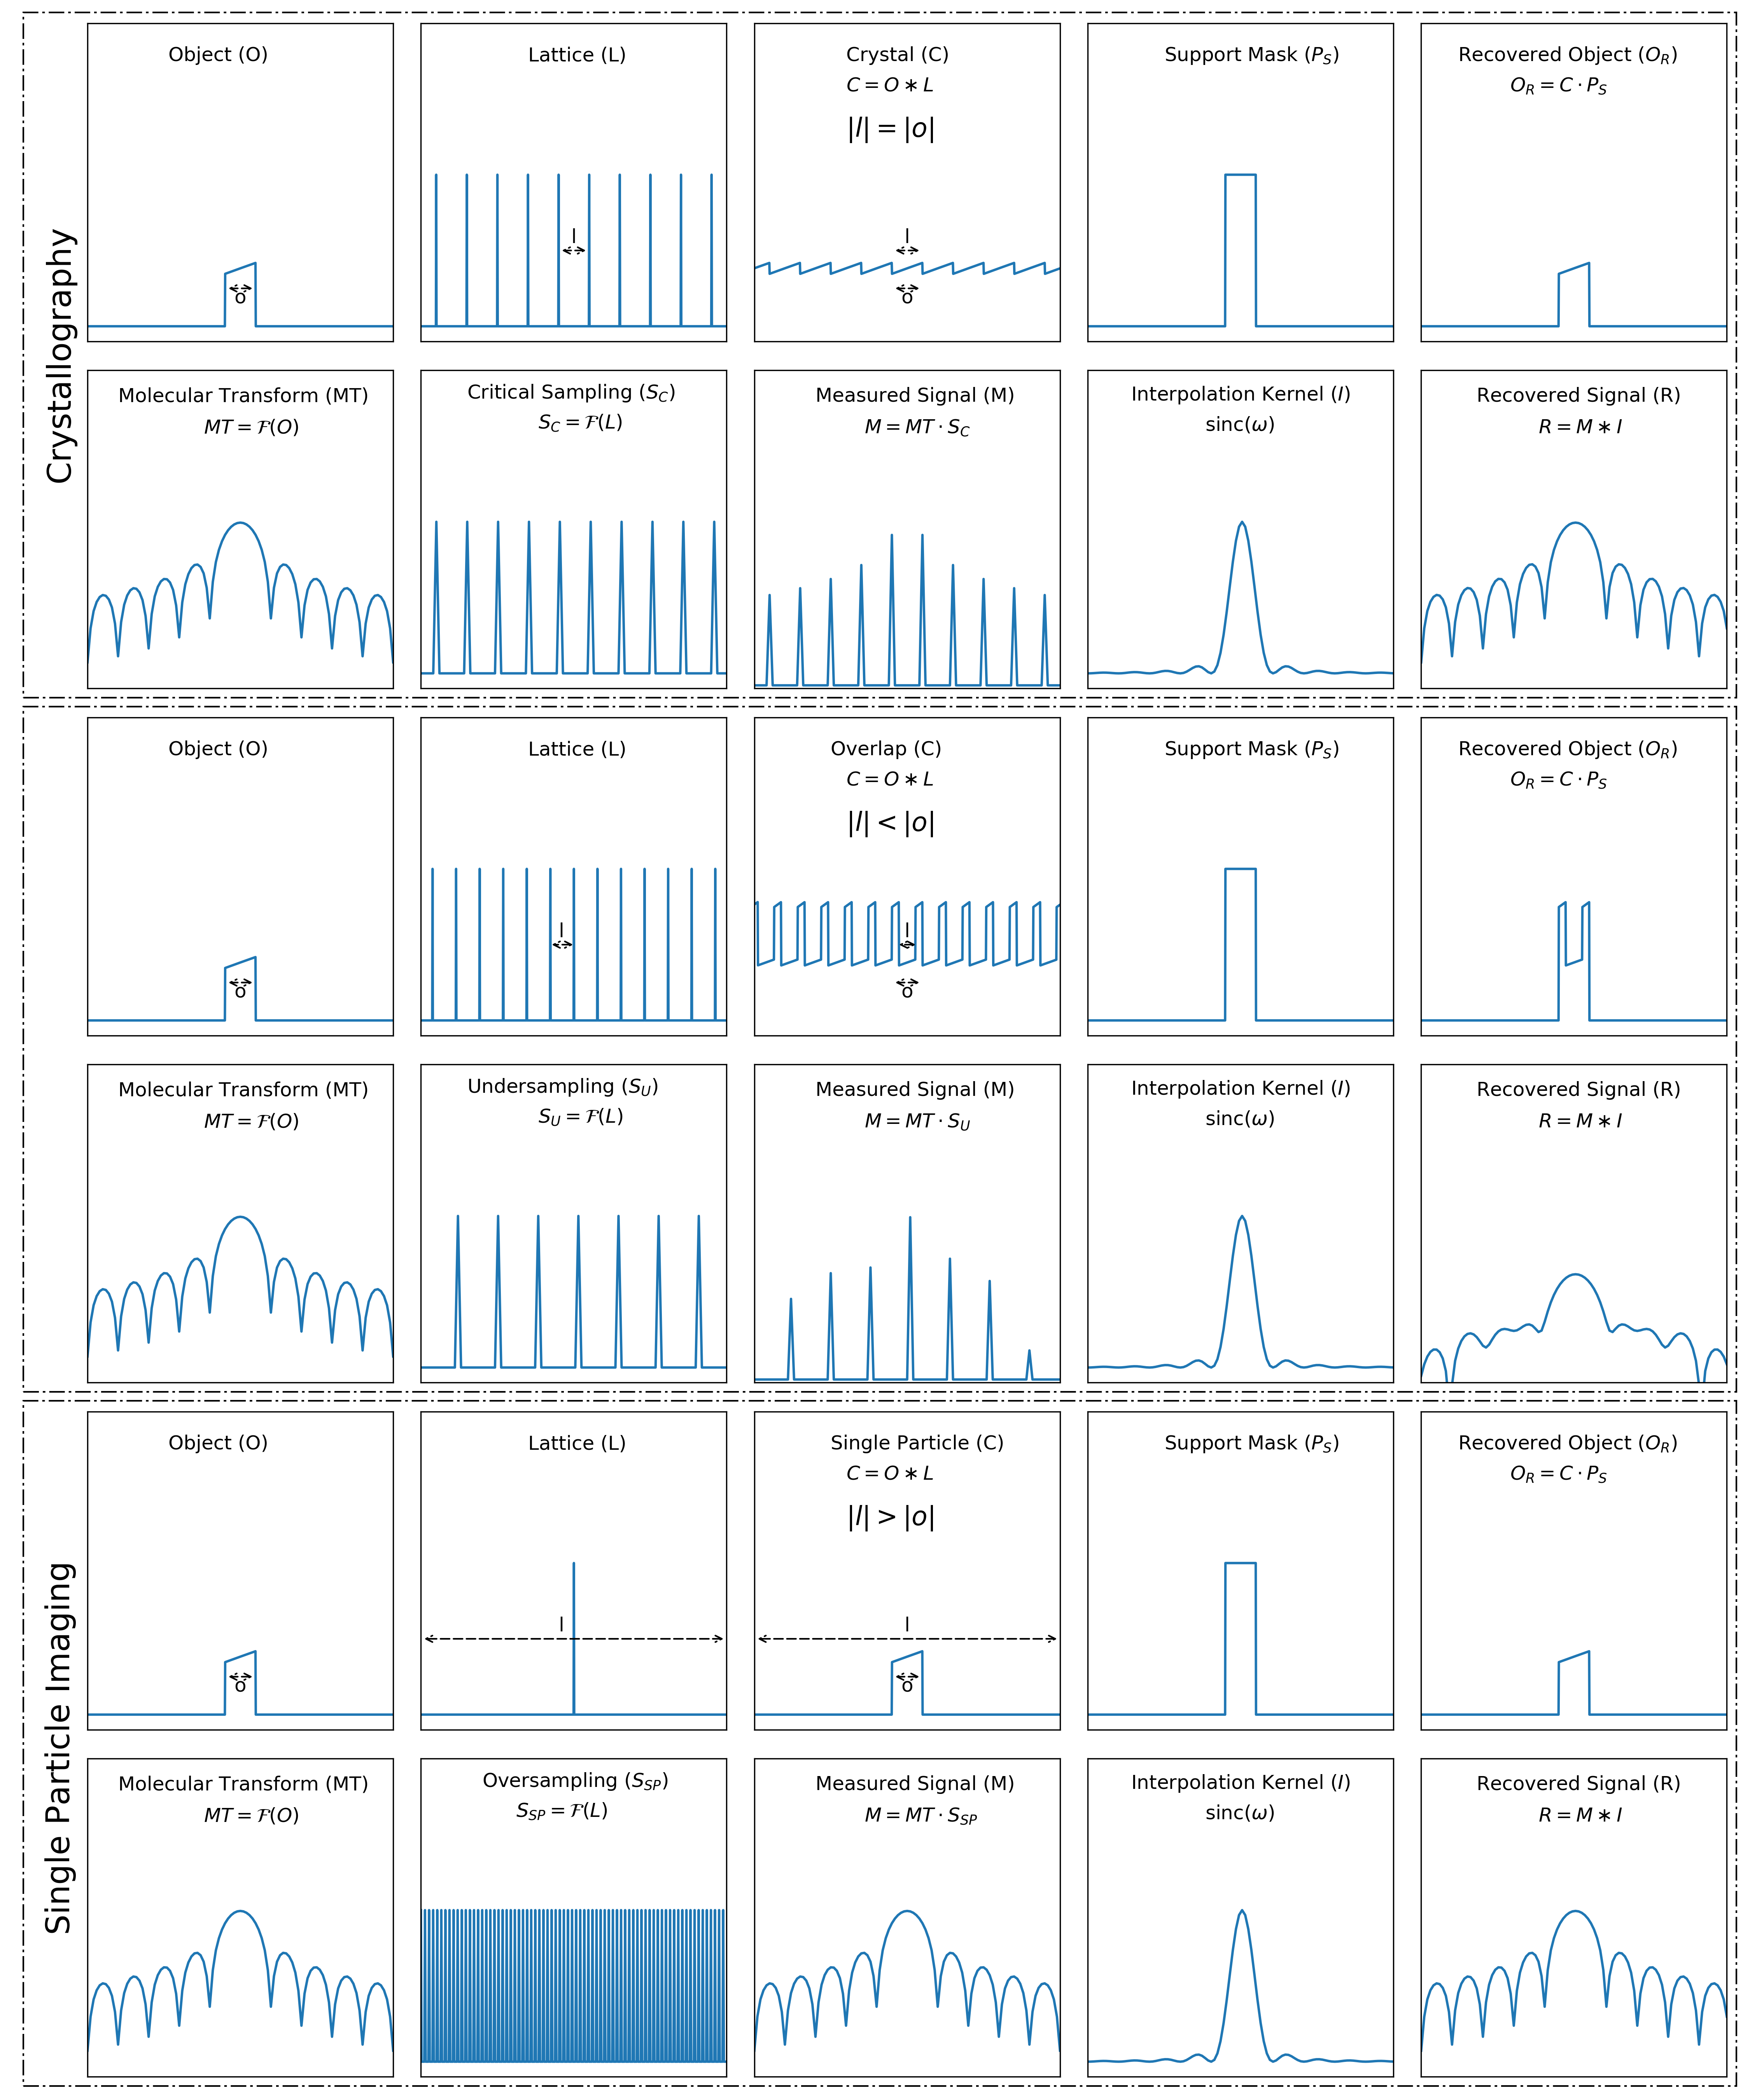
\includegraphics[width=120mm]{SamplingTheory.png}
\caption{Different rates of sampling explained}
\end{figure} 

We collected diffraction patterns of C. gracile cells for 60 minutes at a hit ratio of 43\% and selected the 7,500 clear single hits for further analysis, using the Cheetah software package. The oversampling rate of the particle was around 12-fold, which allowed direct phase recovery from the measured intensity patterns. This was not a trivial problem because strong hits saturate the detectors at low diffraction angles. As a compromise, we selected medium-strong hits, which contained either no, or only few saturated pixels while still providing scattered signal to reasonably high resolution. Missing mode analysis revealed no unconstrained modes for all cells presented in paper I. 

Figure 2 a-j shows the reconstructed exit wave-fronts (images) for ten live C. gracile cells together with the corresponding diffraction patterns, and a synthetic DIC image. The reconstructions represent 2D projections of the electron density of the cells. The images are arranged by increasing size, and show the expected morphologies of cells during division [Komarek,Komarek2]. The resolution of each  reconstruction is indicated by the size of the round white dot. Features smaller than the dot need to be interpreted with care.

Phases were retrieved using the Hawk software package. For each pattern 400 reconstructions were made, each starting from different random initial phases. These reconstructions consisted of 5000 iterations with the RAAR algorithm [Luke], using a Shrinkwrap algorithm[Machesini] for support determination, and concluded with 100 iterations by the ER algorithm[Fienup, Gerchberg-Saxton]. The initial and final support size was selected manually. No additional constraints were used since we anticipated the effects of absorption in the thick cells to give effects similar to a phase object. 

Resolution for the reconstructions was estimated from the PRTF (See Figure \ref{fig:ExperimentalSetup}), using the 1/e cutoff. Before calculating a PRTF and averaging the images we removed outliers among the reconstructions by applying a threshold to the Fourier error. Clustering validates the results from using a threshold on the Fourier-Error and the real-space error(Figures 7 a-j). On average the main cluster contained about 370 out of 400 reconstructions (93), except for one case where only 96 reconstructions formed the biggest cluster (Figure 7j). This made us believe that the average image of the main cluster is the true reconstruction minimum. Th failed reconstructions did not find the true minimum.
The scatter plots of Figure 7 a-j show that the real-space error is more reliable than the Fourier-error for identifying failed reconstructions. Furthermore, clustering aids in the identification of failed reconstructions, as it does for reconstruction 7, even if the error measures are not different. 

Detector saturation limited the achievable resolution.  In fact, the reconstructions shown in Figure \ref{fig:ExperimentalSetup} come from exposures that did not saturate the detectors. A number of much stronger exposures were also recorded, and in some of these exposures the diffraction signal extended to nanometer resolution. Figure \ref{fig:ExperimentalSetup} shows one such pattern for a live S. elongatus cell at 1,100 eV photon energy, 70 fs pulse length, about $10^11$ photons $\mu m^{-2}$ on the sample. Four pnCCD detectors were used to record this pattern (Figure \ref{fig:ExperimentalSetup}b). The configuration of the central back detector in Figure 4 is identical to the detector used in Figure 2. The front detector is the same type as the back detector but is placed at 220 mm from the interaction region. In this strong hit, a large part of the back detector was saturated, preventing reliable phasing. The signal however extended beyond 4 nm resolution on the front detectors (at sigma 3.7), which is the size of a small protein molecule. More than 58 million scattered photons were recorded on the back detectors, and 1.3 million on the front detectors. The size of the cell was derived from the autocorrelation. Figure 4c shows that in a log/log representation the drop-off of the signal is linear with spatial frequency in the range covered by our measurements, and the exponent of the signal decay is $-3.31\pm0.01$, matching simulations [Jakobson].

DICUSSION 

\section{Classification}

Sizing diffraction pattern
\\
Sizing Autocorrelation
\\
Identification multiple scatterers
\\	1) Multiple Particles
\\	2) Holographic Images
\\
Edge detection
\\
Particle shape detection
\\	1) Round particles
\\	2) Elongated Particles
\\
Success on wide variety of sizes and scattering strengths.
\\
Template-based Classification
\\

\section{Software}

\chapter{Sammanfattning pa Svenska}

In this thesis we want to develop new methods to image biological diversity at the molecular level. Understanding this diversity is very important as it can play a major role in development of deceases. The thesis focuses on two topics: the imaging \textit{living} cells and the development of a computational tool to assess variability within a population of images.
\\\\
In molecular biology structure and function are closely related. This however does not mean that each object has one single static shape, as for example a key has. On the contrary, many objects have multiple conformations and only through understanding the variation, their function becomes interpretable. A further complication arises from the fact that the variation is often highly dependent on the exact environment the objects are in. Outside of their natural environment, molecular machines might start operating differently. A tool that can images molecular machinery inside living cells (this is their natural environment) is therefore required to truly understand the structure of molecular life.
\\\\
The amount of detail within objects (resolution) that one can image is limited by the wavelength of the light. Molecular machines are build up out of atoms, so light with a wavelength of the size of an atom is needed understand the functioning of molecular machines. This type of light is X-ray radiation. Another fundamental principle is that the smaller an object is, the stronger the beam of light that shines on the object needs to be in order to record enough information to record an image. Strong beams have the disadvantage that they damage the objects themselves. This led to the limitation that single objects smaller than 100 atoms in diameter could not be resolved structurally with X-rays.
\\\\
The development of a new type of X-ray laser, x-ray free-electron lasers, created the solution to the damage-imposed resolution limit. XFELs produce ultra-short and extremely brilliant X-ray pulses at repetition rates up to 1 billions images a day. The power of the pulse ensures that even individual molecular machines can be imaged in atomic detail. These pulses do damage the objects they image, but because they are ultra-short the damage only happens after the pulse. The recorded image is therefore an image of the undamaged object. This principle is called diffract-before-destroy. 
\\\\
The word diffract indicates that we are not recording images of an object in the way a photo camera captures images. Instead we measure a so called diffraction pattern. The 2D diffraction pattern can be converted to a real image (2D) in a process called image reconstruction. The feasibility of the diffract-before-destroy principle as well as the image reconstruction process has been shown for a variety of non-biological and biological samples in 2D.  And recently the first 3D model of a biological object has been generated from many 2D diffraction patterns.
\\\\
In 2008, researchers showed that it is theoretically possible to image small living cells at sub-nanometer resolution in 2D. The main work of the thesis was an experimental verification of this prediction. It showed that, using a relatively weak XFEL compared to the predicted parameters, it is possible to record images with signal upto 40 atoms resolution. Unfortunately, due to detector saturation, image reconstruction was not successful for these images. To avoid saturation the pulse power had to be limited, which in turn posed the limit to resolution of the recovered object to 82 nm. We have suggested improvements to avoid detector saturation, but these suggestions have not been tested experimentally.
\\\\
Due to the variability between different cells it is not trivial to fully automate the process of object recovery from the recorded image, something that is needed if one want to study the variability of cells, or the molecular machines inside them. For the automation to succeed it necessary to predict the shape of the object from the recorded image itself. Furthermore, other parameters such as saturation or having two cells in the beam at once also have to automatically assessed.
\\\\
This led to the development of the software suite called RedFlamingo. Red Flamingo can be used to assess the quality of individual images, and deduces several essential features for image reconstruction. In some cases it can also determine whether the observed variety originate from a biological source, or whether it is a result from he experiment. It turns out that this feature can be useful in the process of deriving a 3D model from many 2D images. 
\\\\
I am very excited to see the development of this technique. Measuring images without saturation effects might open the door to observing the biological processes occurring inside living cells. As the field is heading now, the initial focus will most likely be on the elucidation of conformational variability in isolated molecular machines. After this we can hopefully observe these machines acting and interacting inside their natural environment, allowing us to visualize the organisation of life.
